
\title{Efficient utilisation of postage batches in Swarm}


\author{assignment for research team candidates}
\date{\today}
\begin{document}
\maketitle
\vspace{.5cm}
\begin{center}

\includegraphics[width=0.2\textwidth]{fig/logo.pdf}
\end{center}
\vspace{1.5cm}

\maketitle
\begin{abstract}
    This assignment is supposed to be self contained. In order to understand the context and motivation behind the problem, we provide quite a verbose introduction to postage stamps and swarm's distributed storage model.
\end{abstract}
\tableofcontents
\newpage
\section{Postage stamps}\label{sec:postage-stamps}

A postage stamp is a verifiable proof of payment associated with a chunk witnessed by the signature of the owner. On the one hand, postage stamps  prevent frivolous uploads by imposing an advance cost. On the other hand, they signal a chunk's relative importance that storer nodes can then use to rank chunks when selecting which ones to retain and serve, and which ones to garbage collect in the event of capacity shortage.


\begin{figure}[htbp]
\centering
  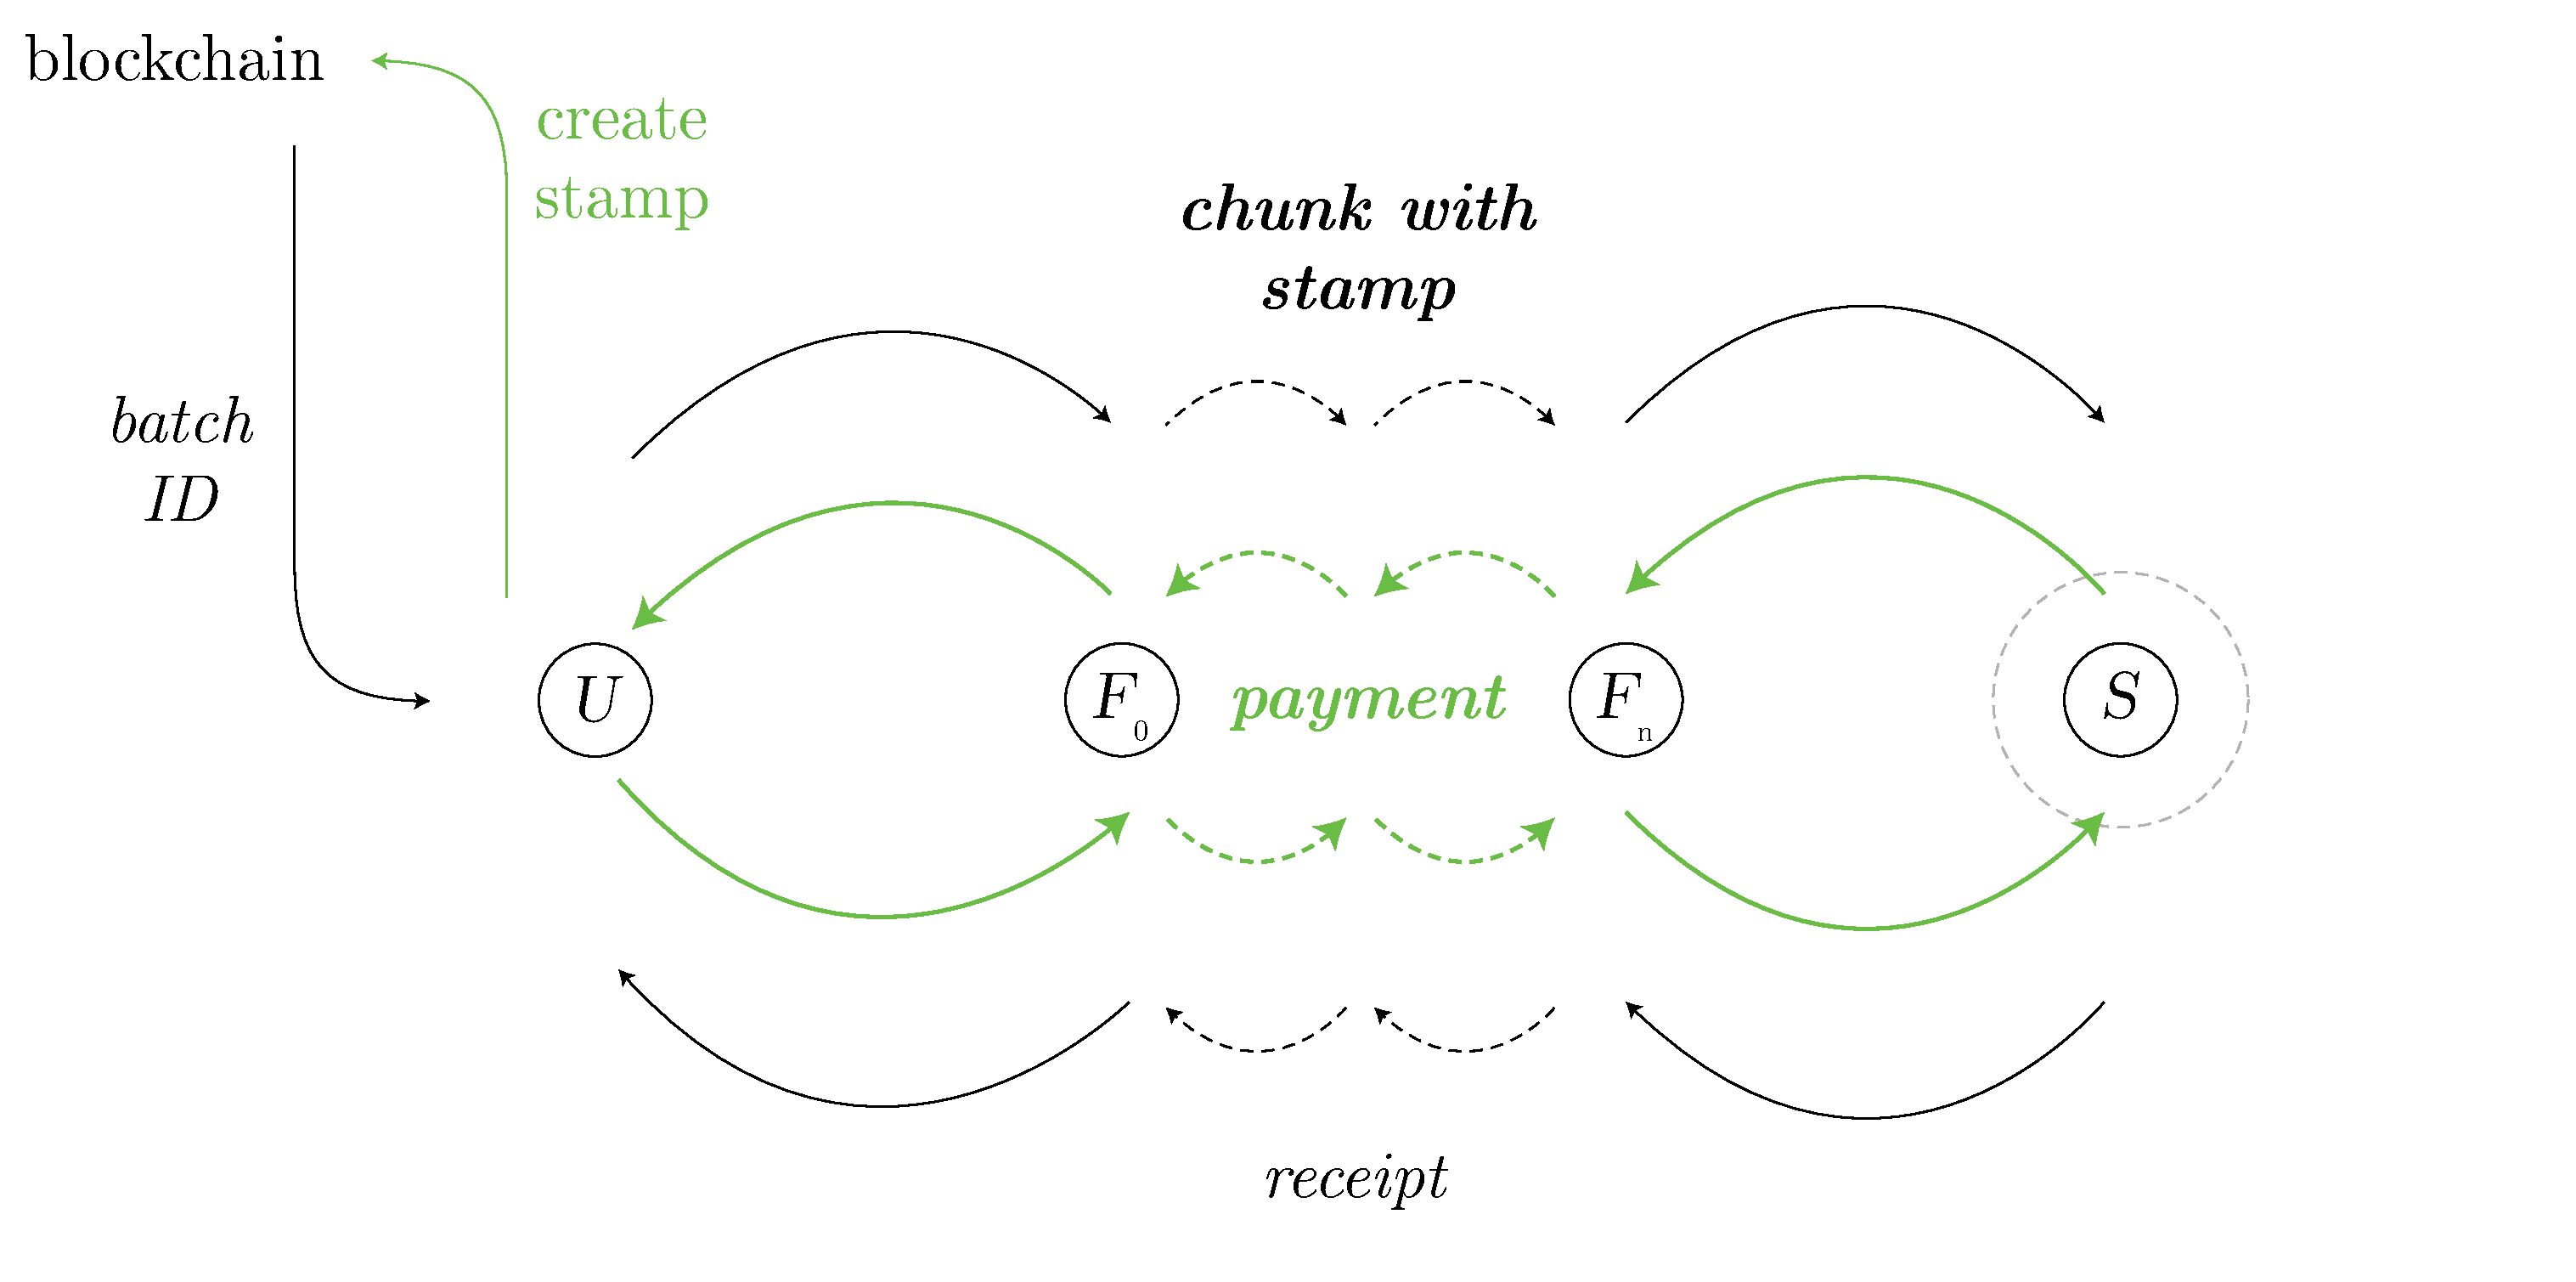
\includegraphics[width=\textwidth]{fig/postage-stamp.pdf}
\caption[Postage stamps]{Postage stamps}
\label{fig:postage-stamps}
\end{figure}

\section{Purchasing a postage batch}

Uploaders purchase the postage stamps in  a  \emph{postage batch} from the postage smart contract on the Ethereum blockchain. Postage batches are created by this contract when a transaction is sent to its creation endpoint, together with an amount of BZZ tokens and the following transaction data:

\begin{itemize}[noitemsep]
\item \emph{owner address} -- The owner that is entitled to use the batches created to stamp chunks.
\item \emph{batch depth} -- Base 2 logarithm of the number of chunks that can be stamped with the batch created.
\end{itemize}

As the transaction executes, a new batch entry is added to the contract storage with the following pieces of information:

\begin{itemize}[noitemsep]
\item \emph{batch identifier} -- A random ID that is generated as reference for this payment.
\item \emph{per-chunk balance} -- The total amount, equally allocated for each chunk covered by this payment.
\item \emph{owner address} -- Ethereum address of the owner that is entitled to use the batch created to stamp chunks.
\item \emph{batch depth} -- Base 2 logarithm of the number of chunks that can be stamped with the batch created.
\item \emph{mutability} -- A boolean flag indicating if the storage slots of the batch can be reassigned 
\end{itemize}


A random identifier is generated to provide a reference to the batch and its depth is recorded for each batch separately. The amount of BZZ tokens sent with the transaction is then allocated equally to all storage slots covered by the payment. This is represented by a per-chunk balance. 
The owner is the Ethereum address that is specified in the transaction data and recorded as the party authorised to use the batch created to stamp chunks; if not specified, it is assumed to be the transaction sender by default. 
Anyone can then choose to top up this balance at a later date. 


\begin{figure}[htbp]
  \centering
    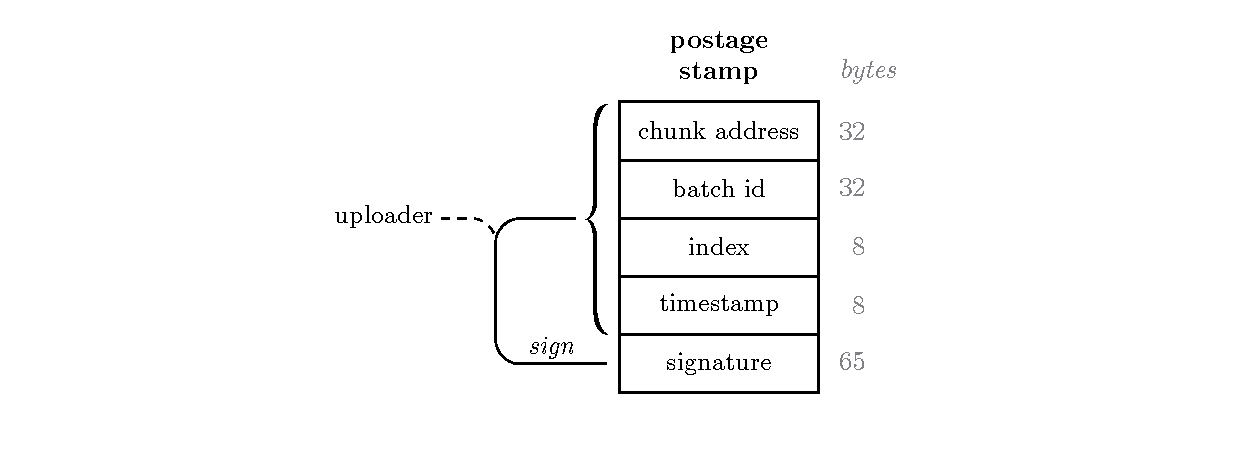
\includegraphics[width=\textwidth]{fig/postage-stamp-structure.pdf}
  \caption[Postage stamp]{Postage stamp is a data structure comprised of the postage contract batch id, storage slot index, timestamp the chunk address and a witness signature attesting to the association of these four. Uploaders and forwarders must attach a valid postage stamp to every chunk uploaded. }
  \label{fig:postage-stamp}
\end{figure}

\section{Stamp validity}

The postage stamp attached to a chunk is a data structure comprising the following fields (see figure  \ref{fig:postage-stamp}):

\begin{itemize}[noitemsep]
    \item \emph{chunk address} -- The address the stamp is attached to. 
    \item \emph{batch identifier} --  A random ID that is generated as reference for this payment.
    \item \emph{storage slot} -- A within-batch index referencing a storage slot
    \item \emph{timestamp} -- The time the chunk is stamped. 
    \item \emph{witness} -- The owner's signature, linking the storage slot and the chunk.
\end{itemize}

\begin{definition}[Postage stamps \statusgreen]
\label{def:postage-stamp}

\begin{equation}
\mathit{ps} \defeq \langle  b,i,ts,a\rangle\in \mathit{Stamps} 
\end{equation}
\begin{eqnarray}    
\mathit{batchID}(ps) &\defeq& b \in\mathit{Segment}
\\
\mathit{count}(ps) &\defeq &i \in\mathit{uint64}
\\
\mathit{timestamp}(ps)&\defeq &ts \in\mathit{Timestamp}
\\
\mathit{address}(ps) &\defeq &a \in\mathit{Address}
\end{eqnarray}

\end{definition}


\begin{definition}[Storage slot reference \statusgreen]
\label{def:slot}
Define the \emph{storage slot reference} $\mathit{slot}(ps)$ of a postage stamp $ps$ as the tuple of the batch identifier and the within-batch stamp counter.
\begin{eqnarray}
\mathit{slot}&:& \mathit{Stamps}\mapsto\mathit{Slots}\\
\mathit{Slots}&\defeq&\mathit{Segment}\times\mathit{uint64}\\
\mathit{slot}(ps) &\defeq &\langle batchID(ps),count(ps)\rangle 
\end{eqnarray}

Naturally storage slot reference of a chunk $slot(c)$ is defined as the slot reference of the postage stamp attached to the chunk.
\end{definition}



A postage stamp's validity can be checked by verifying that it scores all true on the following four attributes::

\begin{itemize}[noitemsep]
\item \emph{authentic} -- The batch identifier is registered in the postage contract's storage.\\ 
Otherwise \texttt{Error:\,not found}
\item \emph{authorised} -- The postage stamp is signed by the address specified as the owner of the batch.\\
Otherwise \texttt{Error:\,not authorised}
\item \emph{available} -- The referenced storage slot is within range given the batch depth, and, in case of an immutable batch, has no duplicates.\\
Otherwise \texttt{Error:\,invalid storage slot}, 
\texttt{Error:\,duplicate slots on   immutable batch}
\item \emph{alive} -- The referenced batch has not yet exhausted its balance.\\
Otherwise \texttt{Error:\,expired}
\end{itemize}

All this can be easily checked by the nodes themselves using the smart contract.

\begin{definition}[Postage stamp validity \statusgreen]
\label{def:postage-stamp-validity}
Define $\mathit{Valid}[\textsc{\lowercase{STAMP}}](ps)$ as the validator of the proof of relevance expressed as the postage stamp $ps$ relying on blockchain information.

\begin{eqnarray}
\mathit{Valid}[\textsc{\lowercase{STAMP}}] &:& \mathit{Stamps} \mapsto \{\mathtt{T,F}\}\\
\mathit{Valid}[\textsc{\lowercase{STAMP}}](ps) &\Leftrightarrow& \\
\textsc{authentic} & & \mathit{batchID}(ps)\in\mathrm{Batches}\wedge
\\
\textsc{authorised} & &  \mathit{ECRecover}(\mathit{Sig}(ps), \mathit{encode}(ps)) = \mathrm{Owner}(ps) \wedge
\\
\textsc{available} & & 0 <= \mathit{Slot}(ps) < \mathit{exp}_2({\mathrm{Depth}(ps)})\wedge
\\
\textsc{alive} & & \mathrm{Balance}(ps) > 0
\end{eqnarray}
\end{definition}


\begin{definition}[valid storage slots]
Define $\mathrm{Size}(b)$, the blockchain's view at block $b$ of the size of reserved capacity as the total number of storage slots by all batches valid at block $b$.
\begin{eqnarray}
\mathrm{Size}&:&\mathit{Blocks}\mapsto \mathit{uint64}\\
\mathrm{Size}(b)&\defeq&\Sigma_{b\in \mathit{Batches}}\mathrm{size}(b)
\end{eqnarray}
\end{definition}


\begin{definition}[reserve radius]
Define $\mathrm{ReserveRadius}(b, nc)$, the blockchain's view at block $b$ of the desired neighbourhood depth as the base 2 log of number of neighbourhoods needed to provide redundant storage for the total number of storage slots by all batches valid at block $b$ given a fixed node capacity of $nc$ chunks.

\begin{eqnarray}
\mathrm{ReserveRadius}&:&\mathit{Blocks}\times\mathit{uint64}\mapsto \mathit{uint8}\\
\mathrm{ReserveRadius}(b)&\defeq&\mathit{log}_2\frac{\mathrm{Size}(b)}{\texttt{NodeCapacity}}
\end{eqnarray}
\end{definition}



\section{Limited issuance}

Purchasing a postage batch effectively entitles the owner to issue postage stamps against the batch ID. The per-chunk balance only makes sense if the batch size, i.e., number of storage slots, is fixed in advance. Batch sizes are restricted to the powers of 2, and specified with its base 2 logarithm, called \emph{batch depth}. Storage slots of a batch with depth $d$ are supposed to be indexed from 0 to $2^d$. The batch size limitation is equivalent to the conditions that the maximum index is $2^d-1$ and there are no duplicate indexes.  

We add to this the constraint that overissuance should be locally verifiable by storer nodes. This boils down to an explicit \emph{uniformity requirement} and an indexing convention for the postage stamp usage. 

The uniformity requirement states that issuance seen in one neighbourhood can be extrapolated to other neighbourhoods. This means that if the batch is overissued in any neighbourhood, the entire batch is considered overissued and storer nodes can legitimately remove excess chunks. In order to keep their chunks safe,  uploaders need to maintain counters for how many stamps they have issued for a neighbourhood and not to issue more than the volume allowed for any one neighborhood.
If they want their chunks preserved, bucket depth should be deeper than the neighbourhood depth (reserve radius) at any point during the lifetime of the batch. For longer term storage when we must be prepared for network growth and increasing depths, this means a deeper bucket depth is required. On the other hand, a shallower bucket is easier to fill efficiently.


 


In order for collisions to be detectable, the collision depth must not be less  than the  neighbourhood depth.
As long as this is maintained, all chunks in the same collision bucket are guaranteed to land in the same neighbourhood, and, as a result, duplicate assignments can be locally detected by nodes (see figure \ref{fig:prefix-collision}).
We can however turn this around and say that, if the collision depth (as deduced from the length of the prefix shared by the chunk address and the storage slot index) is less than the reserve depth, the stamp is regarded as invalid.
To conclude, using uniform storage slots and validating availability protects against \emph{overissuance} using only information available locally to storage nodes. 



\begin{figure}[!ht]
  \centering
    \scalebox{0.8}{
\begin{forest}
slot/.style={rectangle,minimum width=9mm, minimum height=9mm},
filled/.style={fill=lightgray},
mid/.style={circle, radius=1mm},
[{},mid,for tree={draw, grow=south}
  [{},mid,edge label={node[midway,left] {0}}
    [{},mid,edge label={node[midway,left] {0}}
      [{},mid,edge label={node[midway,left] {0}}
        [{$0$},slot,edge label={node[midway,left] {0}}]
        [{$1$},slot,edge label={node[midway,right] {1}}]
      ]
      [{},mid,edge label={node[midway,right] {1}}
        [{$2$},slot,edge label={node[midway,left] {0}}]
        [{$3$},slot,edge label={node[midway,right] {1}}]
      ]
    ]
    [{},mid,edge label={node[midway,right] {1}} 
      [{},mid,edge label={node[midway,left] {0}}
        [{$4$},slot,edge label={node[midway,left] {0}}]
        [{$5$},slot,rectangle,filled,edge label={node[midway,right] {1}}
            [{\footnotesize $1010...$},  l=2mm, rectangle, draw=none, edge=dotted]
        ]
      ]
      [{},mid,edge label={node[midway,right] {1}}
        [{$6$},slot,edge label={node[midway,left] {0}}]
        [{$7$},slot,edge label={node[midway,right] {1}}]
      ]
    ] 
  ]
  [{},mid,edge label={node[midway,right] {1}}
    [{},mid, edge label={node[midway,left] {0}}
      [{},mid,edge label={node[midway,left] {0}}
        [{$8$},slot,filled, edge label={node[midway,left] {0}}
            [{\footnotesize $1000...$}, l=2mm, rectangle, draw=none, edge=dotted]
        ]
        [{$9$},slot,edge label={node[midway,right] {1}}]
      ]
      [{},mid,edge label={node[midway,right] {1}}
        [{$10$},slot,edge label={node[midway,left] {0}}]
        [{$11$},slot,edge label={node[midway,right] {1}}]
      ]
    ]
    [{},mid,edge label={node[midway,right] {1}} 
      [{},mid,edge label={node[midway,left] {0}}
        [{$12$},slot,edge label={node[midway,left] {0}}]
        [{$13$},slot,filled,edge label={node[midway,right] {1}}
            [{\footnotesize $1011...$},  l=2mm, rectangle, draw=none, edge=dotted]
        ]
      ]
      [{},mid,edge label={node[midway,right] {1}}
        [{$14$},slot,edge label={node[midway,left] {0}}]
        [{$15$},slot,edge label={node[midway,right] {1}}]
      ]
    ]
  ] 
]
\end{forest}
}
  \caption[Postage Stamp Priority]{Postage Stamp Priority}
\label{fig:prefix-collision}
\end{figure}    



In general, the most efficient utilisation of a batch is by filling each collision bucket fully.

In practice, full utilisation is defined by one collision bucket completely filled. When items are assigned to buckets with a uniform distribution, as total item count vs bucket count ratio increases, the variance of item counts across buckets decreases. This means that the expected utilisation rate of the other buckets when the first bucket gets full converges to 100\%.

Targeted issuance, continued non-uniformity will lead to underutilised batches, and therefore a higher average unit price for uploading and storing each chunk. This solution has the desired side effect that it imposes an upfront cost to non-uniform uploads: the more concentrated the distribution of chunks of an upload is, the more slots of the postage stamps remain unused. In this way, we ensure that targeted DoS attacks against a neighbourhood (uploading disproportionate number of chunks in a particular address range) is costly since the degree of underutilisation (inert cost) of a batch is exponential in the depth of the skew.


\section{Reserve and cache}\label{sec:reserve}

Beyond DoS protection, postage stamps can serve as a fiduciary signal indicating how much it is worth for a user to persist a chunk in Swarm. In particular, the per-chunk balance of batches can provide the differential a priori bias determining which chunks should be protected from garbage collection in the absence of evidence to predict their profitability. 

The \emph{reserve} is a fixed size of storage space dedicated to storing the chunks in the node's \emph{area of responsibility}. Chunks in the reserve are the chunks that are protected against garbage collection. The content of the reserve is coordinated under consensus with a price oracle and a prescribed reserve capacity. The method determining which chunks should be prevented from deletion is described next.

% \subsection{Batch balance, rent and expiry}


The normalized balance of a chunk is calculated as the batch inpayment divided by batch size. The chunk balance is interpreted as an amount pre-committed to be spent on storage. The balance decreases with time as if \emph{storage rent} was paid for each block at the price dictated by a price oracle contract.  
When batches expire, i.e., their balance is completely depleted, the chunks they comprise get evicted from the reserve and as a result, some reserve space is freed up to accommodate chunks belonging to valid batches.

This system allows prepayment for storage without having to speculate on the future price of storage or fluctuations in the currency's exchange rate. At the cost of decreased certainty about the expiration date, one gains resilience against price volatility. On top of this, uploaders can enjoy the luxury of non-engagement by tying up more of the batch balance; while it serves as collateral against price increase if that does not happen the funds can still be used up (for storing).

From the point of view of incentives, chunks which are of the same proximity order and the same batch are equivalent. When it comes to eviction, these equivalence classes, called \emph{batch bins} are handled as one unit: the chunks in a batch bin are inserted to the garbage collection index in one atomic operation. 

The reserve is governed by the following rules:
\begin{itemize}[noitemsep]
    \item[--] if a batch is reserved on a PO then all batches with a higher value are also reserved
    \item[--] if a batch is reserved on a PO then the same batch is reserved also for all higher POs 
    \item[--] with batch sizes based on fully filled batches, the reserve should not exceed capacity
    \item[--] batch reserve is maximally utilised, i.e, cannot be extended and have 1-3 remain true
\end{itemize}

The preference for closer chunks is incentivised by routing. Keeping the closest chunks, a node will maximise the number of receipts it can issue and the number of retrieve requests it can respond to and at the same time, provides the widest coverage within the neighbourhood even after the neighbourhood is no longer supporting the redundancy for all chunks in neighbourhood. Preference for higher balance is incentivised by higher ultimate profit and hinges on the assumption that balances are not revocable and  ultimately contribute to storers' profit is proportional to their full balance.%
%
\footnote{Note that even if there is no scheme for redistributing postage revenue and the inpayment is frozen/burnt, this strategy is aligned with token-holders interest since batches with higher balance exert more deflationary force on the token (per chunk, i.e, the unit of invested resource) by keeping their balance frozen which is expected to realise in a proportional price increase.}


\begin{figure}[!ht]
  \centering
    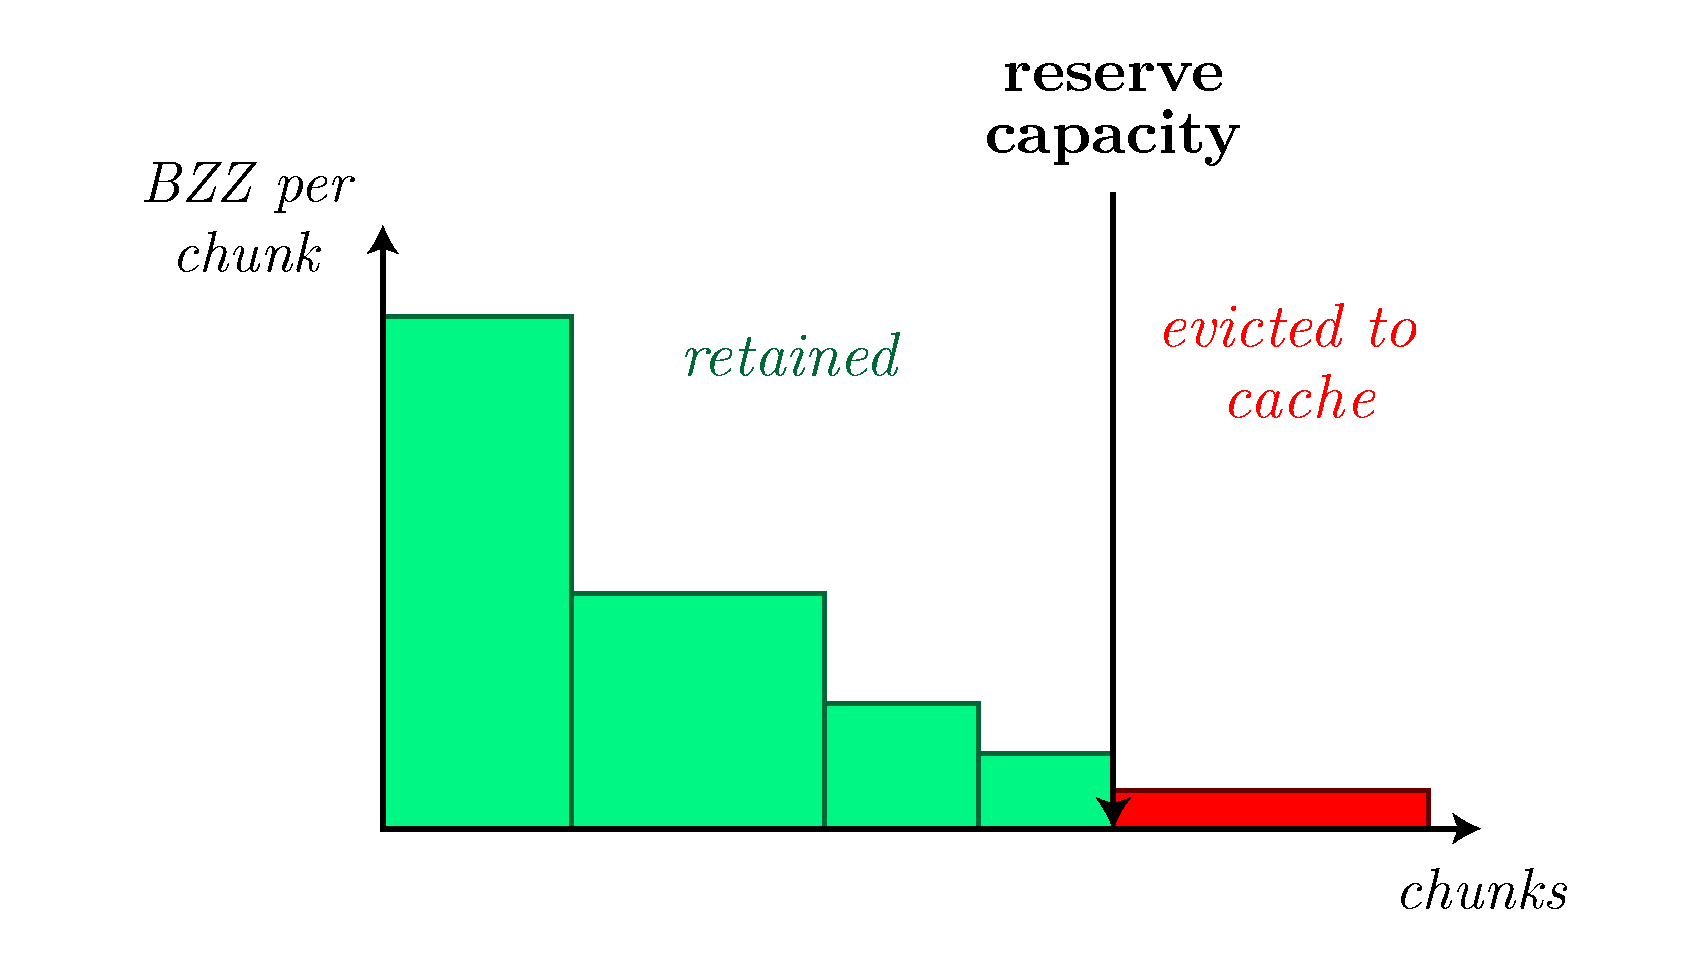
\includegraphics[width=\textwidth]{fig/reserve-capacity-2.pdf}
  \caption[Postage Stamp Priority]{Postage Stamp Priority}
\label{fig:reserve-capacity}
\end{figure}    


% \section{XOR distance and proximity order\statusgreen}\label{sec:proximity}




% \subsection{Proof of storage \statusgreen}
% \subsubsection{Relevance}

\section{Efficient utilisation of postage batches}\label{sec:complexity-filling}

A postage batch is utilised optimally when each of its collision buckets are filled completely. Although hashes are uniform, due to variance one cannot guarantee that $2^d$ independent hashes will always map to the collision buckets of a batch with bucket depth $d$. As a consequence some buckets may fill up earlier than others. Once a bucket is full, there is no guarantee that the batch can be used to stamp just any chunk: if the next chunk to stamp falls in a bucket that is full, the stamping fails. In case  we cannot influence which bucket our stamp falls, then such a batch can no longer serve us.

\section{Questions}

\subsection*{Question 1}
What is the expected utilisation rate of a postage stamp with bucket depth $b$ and batch depth $d$, i.e., one in which each collision bucket can hold $2^{d-b}$ chunks.

 
\subsection*{Question 2}
Once a bucket of a batch is full, we cannot guarantee that any  chunk can be stamped with it. But what if we can then use a new batch of the same parameters and use that as fallback in case the relevant bucket of the first one is full? What is the probability that given bucket depth $b$ and batch depth $d$, keeping a second 'spillover' batch will not be sufficient to store the capacity of one batch (ie., $2^d$ random chunks), in other words, what are the chances that a bucket will get filled in both batches before i stamp all the $2^d$ chunks.

\subsection*{Question 3}

We have presented various ways of mining chunks: by (1) choosing the nonce of a trojan chunk, (2) choosing the encryption key (see \ref{sec:postage-stamps}), or (3) choosing the index of a single owner chunk (see \ref{sec:addressed-envelopes}). Whichever way we are mining chunks, this allows us to choose the bucket for a chunk. Practically, when it comes to filling in postage batches, with each extra cycle of work (mining attempt) we give an extra chance for the chunk to fall in a bucket that is not full.
In fact if we are frugal and want to fill our postage batch to 100\%
utilisation, we can use a strategy that when the next chunk falls in a collision bucket that is already full, we keep mining a new chunk address until it can be accommodated.

The question is, given a batch with bucket depth $b$ and batch depth $d$, what is the expected ratio of extra mining cycles necessary in order to fill the batch $p$ percent full.

What follows can be used as a cheat sheet. It calculates the expected mining overhead for the (sadly irrelevant) special case when $b=d$, i.e., the batch can issue a single chunk per bucket.


\subsection*{Question 4}
Write a simple simulation to model the task of question 3, plot and analyse results.

\newpage
\subsection*{Proof of question 3 for the case when $b=d$}

We may calculate in the chance of finding an address that falls in the $i$-th collision bucket of the stamp, i.e.


\begin{equation}
\mathit{PO}(\mathit{H}(\mathit{Enc}(k, c)), \mathit{CS}(i))\geq\mathit{D},
\text{ where }\mathit{CS}(i)\defeq i*2^{256-D}
\text{ for }0\leq i\leq  2^D.
\end{equation}

If a user wishes to always fill their postage stamp batch before using another one, for each new chunk there is one less choice to pick a free collision bucket. So, let the probability variable $X^n_i$ denote  the number of trials one needed to find a slot when $i$ out of $n$ slots are free. The probability that we will require at least 1 trial is $\frac{n-i}{n}$, and in general:


\begin{equation}\label{eq:conditional}
\mathit{P}(X^n_i\geq j+1|X^n_i\geq j)=\frac{n-i}{n}\\
\end{equation}

Therefore, the expected number of trials for the $i$-th chunk is: 

 \begin{subequations}   \begin{align}
\mathit{E}(X^n_i)&=\sum^\infty_{j=1}j\mathit{P}(X^n_i=j)\\
&=\mathit{P}(X^n_i\geq 1)-\mathit{P}(X^n_i\geq 2)+2(\mathit{P}(X^n_i\geq 2)-P(X^n_i\geq 3))+\ldots\\
&= \mathit{P}(X^n_i\geq 1)+\mathit{P}(X^n_i\geq 2)+\ldots
\end{align} \end{subequations}

Multiplying both sides with $\frac{n-i}{n}$, then using  the equivalence defined in  \ref{eq:conditional} we get:

 \begin{subequations}   \begin{align}
\mathit{E}(X^n_i)\frac{n-i}{n}&=\mathit{P}(X^n_i\geq 1)\mathit{P}(X^n_i\geq 2|X^n_i\geq 1)+\mathit{P}(X^n_i\geq 2)\mathit{P}(X^n_i\geq 3|X^n_i\geq 2)+\ldots\\
&=\mathit{P}(X^n_i\geq 2)+\mathit{P}(X^n_i\geq 3)+\ldots\\
&=\mathit{E}(X^n_i)-\mathit{P}(X^n_i\geq 1)\\
&=\mathit{E}(X^n_i)-\frac{n-i}{n}
\end{align} \end{subequations}

From this, we solve to $\mathit{E}(X^n_i)$:

 \begin{subequations}   \begin{align}
\mathit{E}(X^n_i)(1-\frac{n-i}{n})&=1\\
\mathit{E}(X^n_i)&=\frac{n}{i}
\end{align} \end{subequations}

Averaging for the whole batch ($n=2^d$) gives%
%
\footnote{see harmonic series 
\url{https://en.wikipedia.org/wiki/Harmonic\_series\_(mathematics)\#Rate\_of\_divergence}.}

 \begin{subequations}   \begin{align}
\sum_{i=1}^{2^d}\frac{2^d}{i}\frac{1}{2^d}
&=\sum_{i=1}^{2^d}\frac{1}{i}\\
&=\mathit{ln}(2^d)+1\\
&=\frac{\mathit{log}_2(2^d)}{\mathit{log}_2(e)}+1\\
&=d*0.6931+1
\end{align} \end{subequations}


\end{document}
